\documentclass{beamer}
\usetheme{Copenhagen} % {Malmoe} % {Warsaw} % {Boadilla} % {Madrid}

%% Packages
%-------------------------------------------------------------------------------
\usepackage[utf8]{inputenc}
\usepackage[english]{babel}
\usepackage[absolute,overlay]{textpos}
\usepackage{array}
%\graphicspath{Graphics/}
\usepackage{multimedia}
\usepackage{hyperref}
\usepackage{ulem}
\usepackage{color}
\usepackage{siunitx}
\usepackage{amssymb}
\usepackage{multirow}
\beamertemplatenavigationsymbolsempty


%%%%%%%%%%%% Layout color settings
%-------------------------------------------------------------------------------
\setbeamercolor{normal text}{fg=white,bg=black!90}
\setbeamercolor{structure}{fg=blue!15!black!30}%white}

\setbeamercolor{alerted text}{fg=red!85!black}

\setbeamercolor{item projected}{use=item,fg=black,bg=item.fg!35}

\setbeamercolor*{palette primary}{use=structure,fg=structure.fg}
\setbeamercolor*{palette secondary}{use=structure,fg=structure.fg!95!black}
\setbeamercolor*{palette tertiary}{use=structure,fg=structure.fg!90!black}
\setbeamercolor*{palette quaternary}{use=structure,fg=structure.fg!95!black,bg=black!80}

\setbeamercolor*{framesubtitle}{fg=black!50}

\setbeamercolor*{block title}{parent=structure,bg=black!60}
\setbeamercolor*{block body}{fg=black,bg=black!10}
\setbeamercolor*{block title alerted}{parent=alerted text,bg=black!15}
\setbeamercolor*{block title example}{parent=example text,bg=black!15}

\setbeamercolor{framesource}{fg=black!50}
\setbeamerfont{framesource}{size=\tiny}


%%%%%%%%%%%% Custom commands
%-------------------------------------------------------------------------------
\newcommand{\source}[1]{\begin{textblock*}{7cm}(0.25cm,8.6cm)
 \begin{beamercolorbox}[ht=0.5cm,left]{framesource}
  \usebeamerfont{framesource}\usebeamercolor[fg]{framesource} {#1}
 \end{beamercolorbox}
\end{textblock*}}


%%%%%%%%%%%% Information
%-------------------------------------------------------------------------------
\title{Radiation hydrodynamics of star formation}
\author{Philipp Denzel}
\date{\today}
\institute{Institute for Computational Science}


%%%%%%%%%%%% Presentation
%-------------------------------------------------------------------------------
\begin{document}

{\usebackgroundtemplate{\includegraphics[width=\paperwidth,height=\paperheight]{Graphics/radiation_cover.png}}
\begin{frame}
 \frametitle{Radiation hydrodynamics of star formation}
 \framesubtitle{Infrared feedback in molecular clouds\\Master thesis presentation}
\end{frame}
}
%-------------------------------------------------------------------------------
\begin{frame}
\frametitle{Structure}
%\tableofcontents[currentsection]
\begin{itemize}
  \item Radiation hydrodynamics\\[15pt]
  \item Numerical methods\\[15pt]
  \item Molecular clouds\\[15pt]
  \item Star formation theory\\[15pt]
  \item Simulation results\\[15pt]
\end{itemize}

\end{frame}
%-------------------------------------------------------------------------------
\begin{frame}
\frametitle{Hydrodynamics}
 \begin{itemize}
   \item Particles \quad\:\:---\, Continuum
   \item Microscopic ---\, Macroscopic\\[12pt]
 \end{itemize}
 Euler equations
 \begin{align*}
  \frac{\partial \rho}{\partial t} &+ \nabla\cdot (\rho\textbf{u})= 0 \\
  \frac{\partial (\rho\textbf{u})}{\partial t} &+ \nabla\cdot (\rho(\textbf{u} \otimes \textbf{u}) + \mathbb{P}) = \rho \textbf{a} \\
  \frac{\partial E}{\partial t} &+ \nabla \cdot (E + \mathbb{P}) \textbf{u} = \rho \textbf{a} \textbf{u}
 \end{align*}
\end{frame}
%-------------------------------------------------------------------------------
\begin{frame}
\frametitle{Radiative transfer}
 \includegraphics[width=0.9\paperwidth,decodearray={0.8 0.1}]{Graphics/rt_source_terms.png}
 \source{http://www.cv.nrao.edu/~sransom/web/Ch2.html}
\end{frame}
%-------------------------------------------------------------------------------
\begin{frame}
\frametitle{Radiative transfer}
 Radiative transfer equation
 \begin{align*}
  \frac{1}{c}\frac{\partial I_{\nu}}{\partial t} &+ \hat{\textbf{n}}\cdot\nabla I_{\nu} = j_{\nu} - \alpha_{\nu}I_{\nu} \\
  \frac{\partial E_{\nu}}{\partial t} &+ \nabla\cdot\textbf{F}_{\nu} = 4\pi j_{\nu} - \alpha_{\nu}cE_{\nu} \\
  \frac{1}{c^{2}}\frac{\partial\textbf{F}_{\nu}}{\partial t} &+ \nabla\cdot\mathbb{P}_{\nu} = - \frac{\alpha_{\nu}\textbf{F}_{\nu}}{c}
 \end{align*}
\end{frame}
%-------------------------------------------------------------------------------
\begin{frame}
 \frametitle{Numerical methods}
 \begin{equation*}
   \frac{\partial\textbf{U}}{\partial t} + \nabla \cdot \textbf{F} = \textbf{S} \quad\Rightarrow\quad \textbf{U}_{i}^{n+1} = \textbf{U}_{i}^{n} - \frac{\Delta t}{\Delta x} (\textbf{F}^{n+1/2}_{i+1/2} - \textbf{F}^{n+1/2}_{i-1/2})
 \end{equation*}
 \colorbox{white}{\includegraphics[width=0.8\paperwidth]{../Figures/piecewise_u.pdf}}
\end{frame}
%-------------------------------------------------------------------------------
\begin{frame}
 \frametitle{Adaptive Mesh Refinement}
 \includegraphics[width=0.8\paperwidth]{Graphics/amr_demo.jpg}
 \source{Antepara, O. et al, Computers \& Fluids 110 (2015) 48--61}
\end{frame}
%-------------------------------------------------------------------------------
{\usebackgroundtemplate{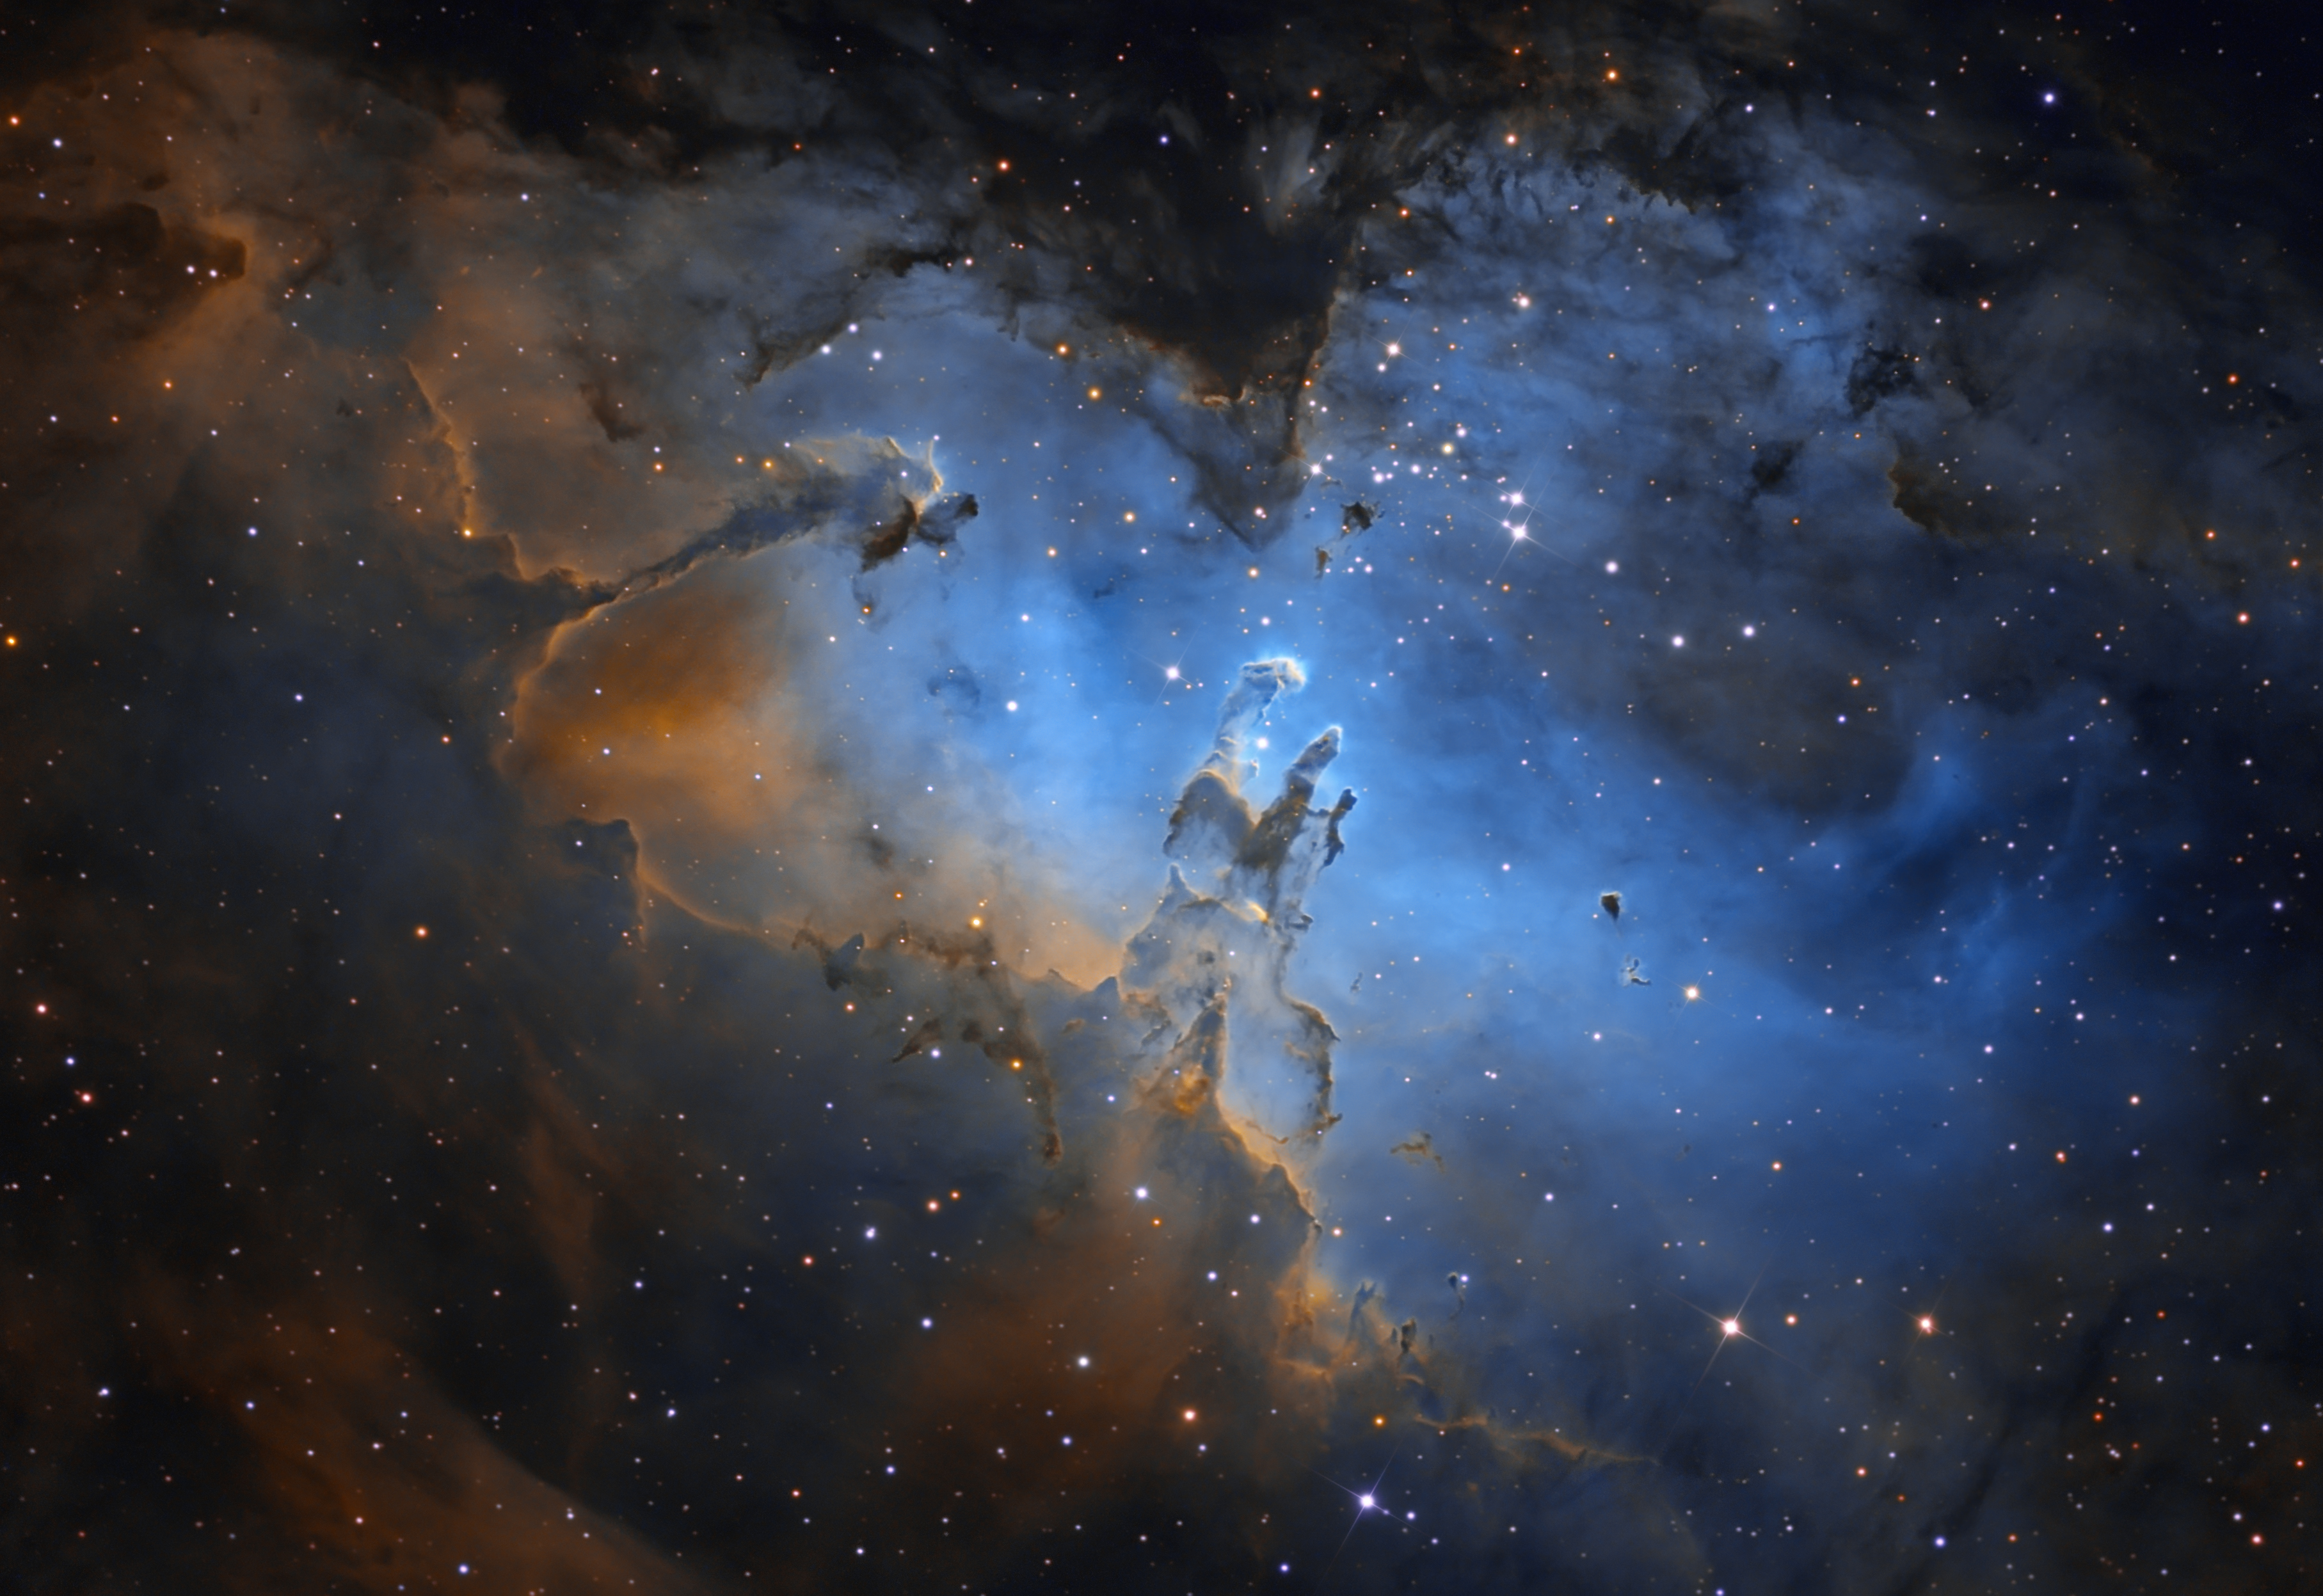
\includegraphics[width=\paperwidth,height=\paperheight]{../Figures/eagle_nebula.jpg}}
\begin{frame}
 \source{http://apod.nasa.gov/apod/image/1510/M16HubbleV4-X3walker.jpg}
\end{frame}
}
%-------------------------------------------------------------------------------
{\usebackgroundtemplate{\includegraphics[width=\paperwidth,height=\paperheight]{../Figures/pillars_of_creation.jpg}}
\begin{frame}
 \source{Credit: NASA, ESA/Hubble and the Hubble Heritage Team\\http://cdn.spacetelescope.org/archives/images/screen/heic1501a.jpg}
\end{frame}
}
%-------------------------------------------------------------------------------
%-------------------------------------------------------------------------------
%-------------------------------------------------------------------------------
\begin{frame}
 \includegraphics[width=0.9\paperwidth,height=0.9\paperheight]{Graphics/larson_cores.png}
 \source{Vaytet, N. et al., A\&A 557, A90 (2013)}
\end{frame}
%-------------------------------------------------------------------------------
%-------------------------------------------------------------------------------
%-------------------------------------------------------------------------------
\begin{frame}
 \frametitle{Core collapse -- pure HD}
 \centering
 \movie[width=0.85\paperwidth,height=0.85\paperheight,loop,showcontrols=false]{\hspace{0.12\paperwidth}\includegraphics[width=0.7\textwidth]{Graphics/play_icon.png}}{Movies/ref_run.mp4}
\end{frame}
%-------------------------------------------------------------------------------
\begin{frame}
 \frametitle{Core collapse -- RHD}
 \centering
 \movie[width=0.85\paperwidth,height=0.85\paperheight,loop,showcontrols=false]{\hspace{0.12\paperwidth}\includegraphics[width=0.7\textwidth]{Graphics/play_icon.png}}{Movies/nsub_const_rtc.mp4}
\end{frame}
%-------------------------------------------------------------------------------
\begin{frame}
\frametitle{Comparison at 20 kyrs}
 \centering
  \includegraphics[width=0.6\paperwidth]{../Figures/hydro_pure/pure_hydro_2.png}\\
  \includegraphics[width=0.6\paperwidth]{../Figures/rhd/multi_00079.png}\\
\end{frame}
%-------------------------------------------------------------------------------
%-------------------------------------------------------------------------------
%-------------------------------------------------------------------------------
\begin{frame}
\frametitle{Toomre analysis}
 \centering
 HYDO \hspace{4cm} RHD\\
 \colorbox{white}{
  \includegraphics[width=0.4\paperwidth]{../Figures/toomre_hydro.png}
  \includegraphics[width=0.4\paperwidth]{../Figures/toomre_rt.png}
 }
\end{frame}
%-------------------------------------------------------------------------------
%-------------------------------------------------------------------------------
\begin{frame}
\frametitle{Simulated molecular cloud}
 \centering
 \movie[width=0.85\paperwidth,height=0.85\paperheight,loop,showcontrols=false]{\hspace{0.12\paperwidth}\includegraphics[width=0.7\textwidth]{Graphics/play_icon.png}}{Movies/dens_.mp4}
\end{frame}
%-------------------------------------------------------------------------------
\begin{frame}
\frametitle{Eddington analysis}
 \colorbox{white}{\includegraphics[width=0.8\paperwidth]{../Figures/cloud_profiles/eddington_limits.pdf}}
\end{frame}
%-------------------------------------------------------------------------------
\begin{frame}
\frametitle{Star cluster}
 \centering
 HYDO \hspace{4cm} RHD\\
 \colorbox{white}{
  \includegraphics[width=0.4\paperwidth]{../Figures/cloud_plots/virial_noRTcloud.pdf}
  \includegraphics[width=0.4\paperwidth]{../Figures/cloud_plots/virial_IRcloud.pdf}
 }
\end{frame}
%-------------------------------------------------------------------------------
%-------------------------------------------------------------------------------
%-------------------------------------------------------------------------------
%-------------------------------------------------------------------------------
\begin{frame}
\frametitle{Thank you for listening!}
 \centering
 \movie[width=0.85\paperwidth,height=0.85\paperheight,loop,showcontrols=false]{\hspace{0.12\paperwidth}\includegraphics[width=0.7\textwidth]{Graphics/play_icon.png}}{Movies/Fp1_.mp4}
\end{frame}
%-------------------------------------------------------------------------------
\begin{frame}
\frametitle{Escapers}
 \centering
 \movie[width=0.85\paperwidth,height=0.85\paperheight,loop,showcontrols=false]{\hspace{0.12\paperwidth}\includegraphics[width=0.7\textwidth]{Graphics/play_icon.png}}{Movies/escapers_IR.mp4}
\end{frame}
%-------------------------------------------------------------------------------
%-------------------------------------------------------------------------------
%-------------------------------------------------------------------------------
% \begin{frame}
% \frametitle{Cloud pressure}
%  \centering
%  \movie[width=0.85\paperwidth,height=0.85\paperheight,loop,showcontrols=false]{\hspace{0.12\paperwidth}\includegraphics[width=0.7\textwidth]{Graphics/play_icon.png}}{Movies/press_.mp4}
% \end{frame}
%-------------------------------------------------------------------------------
\begin{frame}
\frametitle{Cloud temperature}
 \centering
 \movie[width=0.85\paperwidth,height=0.85\paperheight,loop,showcontrols=false]{\hspace{0.12\paperwidth}\includegraphics[width=0.7\textwidth]{Graphics/play_icon.png}}{Movies/temp_.mp4}
\end{frame}
%-------------------------------------------------------------------------------
\end{document}
